\documentclass[11pt,twoside]{report}

 \pagestyle{headings}

\textwidth=440pt
\hoffset=-0.6truein

\usepackage{amsmath}
\usepackage{amsfonts}
\usepackage{amssymb}
%\usepackage{amsthm}
\usepackage{dsfont}
\usepackage{pifont}
%\usepackage{bbold}
\usepackage{graphicx}
\usepackage{epstopdf}
\usepackage{epsfig}
%\usepackage{bibunits}
%\usepackage{theorem}
\usepackage[framed]{ntheorem}
\usepackage{framed}
%\usepackage{showlabels}
\usepackage{makeidx}
\usepackage{simplewick}
\usepackage{tikz-feynman}
\usepackage{slashed}
\usepackage{appendix}

\tikzfeynmanset{compat=1.0.0}  

\newcommand{\tick}{\ding{52}}
\newcommand{\notick}{\ding{56}}
\newcommand{\D}{\displaystyle}
\newcommand{\mphys}{m_\mathrm{phys}}
\newcommand{\tphi}{\tilde{\phi}}
\newcommand{\tj}{\tilde{J}}
\newcommand{\tchi}{\tilde{\chi}}
\newcommand{\psibar}{\bar{\psi}}
\newcommand{\etabar}{\bar{\eta}}
\newcommand{\munu}{{\mu\nu}}
\renewcommand{\chaptername}{Lecture}

\def\bfx{{\mathbf x}}
\def\bfxp{{\mathbf x^\prime}}
\def\bfy{{\mathbf y}}
\def\bfyp{{\mathbf y^\prime}}
\def\bfp{{\mathbf p}}
\def\bfpp{{\mathbf p^\prime}}
\def\ddt{\frac{d}{dt}}
\def\ddtt{\frac{d^2}{dt^2}}
\def\ie{{\it i.e.}\ }
\def\eg{{\it e.g.}\ }
\def\viz{{\it viz.}\ }
\def\matF{\mathcal F}
\def\matE{\mathcal E}
\def\GL{\mathrm{GL}}
\def\kpsi{|\psi\rangle}
\def\kpsione{|\psi_1\rangle}
\def\kpsitwo{|\psi_2\rangle}
\def\kpsionep{|\psi_1^\prime\rangle}
\def\kpsitwop{|\psi_2^\prime\rangle}
\def\kpsii{|\psi_i\rangle}
\def\kpsin{|\psi_n\rangle}
\def\kpsip{|\psi^\prime\rangle}
\def\bpsi{\langle\psi |}
\def\bpsione{\langle\psi_1 |}
\def\bpsitwo{\langle\psi_2 |}
\def\bpsii{\langle\psi_i |}
\def\bpsip{\langle\psi^\prime |}
\def\kphi{|\phi\rangle}
\def\kphione{|\phi_1\rangle}
\def\kphitwo{|\phi_2\rangle}
\def\kphii{|\phi_i\rangle}
\def\kphip{|\phi^\prime\rangle}
\def\bphi{\langle\phi |}
\def\bphione{\langle\phi_1 |}
\def\bphitwo{\langle\phi_2 |}
\def\bphii{\langle\phi_i |}
\def\bphip{\langle\phi^\prime |}
\def\bchi{\langle\chi |}
\def\bchione{\langle\chi_1 |}
\def\bchitwo{\langle\chi_2 |}
\def\bchii{\langle\chi_i |}
\def\bchip{\langle\chi^\prime |}
\def\kjm{|j,m\rangle}
\def\tr{\mathrm{Tr}}
\def\Rn{\mathbb{R}^n}
\def\Cn{\mathbb{C}^n}
\def\id{\mathds{1}}
{\theoremstyle{plain} \theorembodyfont{\rmfamily} \newframedtheorem{Ex}{Exercise}[section]}
{\theoremstyle{plain} \theorembodyfont{\rmfamily} \newframedtheorem{Def}{Definition}[section]}
{\theoremstyle{plain} \theorembodyfont{\rmfamily} \newframedtheorem{Thm}{Theorem}[section]}

\newcommand{\clearemptydoublepage}{\newpage{\pagestyle{empty}\cleardoublepage}}
\newcommand{\HRule}{\rule{\linewidth}{0.5mm}}
\newcommand{\iu}{\underline{i}}
\newcommand{\ju}{\underline{j}}
\newcommand{\ku}{\underline{k}}
\newcommand{\ru}{\underline{r}}
\newcommand{\pu}{\underline{p}}
\newcommand{\Lu}{\underline{L}}
\newcommand{\Ju}{\underline{J}}
\newcommand{\lap}{\nabla^2}
\newcommand{\ad}{\hat{a}}
\newcommand{\ac}{\hat{a}^\dagger}
\newcommand{\re}{\mathrm{Re}}
\newcommand{\ket}[1]{| #1 \rangle}
\newcommand{\bra}[1]{\langle #1 |}
\newcommand{\braket}[2]{\langle #1 | #2 \rangle}
\newcommand{\pref}[1]{(\ref{#1})}
\newcommand{\Eqref}[1]{Eq.~(\ref{#1})}
\newcommand{\del}{\v{\nabla}}				% Underlined del



\makeindex

\begin{document}

\title{Quantum Field Theory}
\author{L. Del Debbio, University of Edinburgh \\
  Version 0.1}

\pagenumbering{roman}
\maketitle
\clearemptydoublepage
\tableofcontents
\clearemptydoublepage

\pagenumbering{arabic}

\chapter{Introductory Thoughts}
\label{chap:intro}
This is introductory material.


\chapter{Gaussian Integrals}
\label{chap:lec0}
\section{Multidimensional Gaussian Integrals}
\label{sec:mult-gauss-integr}

Consider the $n$-dimensional integral
\begin{equation}
  \label{eq:GaussIntOne}
  Z_A = \int d^nx\, \exp\left(
    -\frac12 \sum_{i,j=1}^n x_i A_{ij} x_j
    \right)\, .
\end{equation}
If $A$ is a complex, symmetric $n\times n$ matrix such that
\begin{align}
  & \re\ A \geq 0 \, ,\\
  & a_i \neq 0\, , \quad a_i\ \text{e.vals of }\ A\, ,
\end{align}
then 
\begin{equation}
  \label{eq:GaussIntTwo}
  Z_A = \left(2\pi\right)^{n/2} \left(\det A \right)^{-1/2}\, .
\end{equation}

\paragraph{General Gaussian Integral}

\begin{align}
  Z_A(b) &= \int d^nx\, \exp\left(
  -\frac12 \sum_{i,j=1}^n x_i A_{ij} x_j
  + \sum_{i=1}^n b_i x_i
  \right) \\
  \label{eq:GaussIntThree}
  &=  \left(2\pi\right)^{n/2} \left(\det A \right)^{-1/2}
    \exp\left(
  \frac12 \sum_{i,j=1}^n b_i \Delta_{ij} b_j
  \right) \, ,
\end{align}
where $\Delta = A^{-1}$. The existence of $\Delta$ is guaranteed by the non-vanishing e.vals of $A$.
\begin{Ex}
  Check the result in Eq.~\ref{eq:GaussIntThree} by changing the integration variables in the integral:
  \[
    x_i = y_i + \sum_{j=1}^n \Delta_{ij} b_j\, .
  \]
\end{Ex}

\section{Generating function}
\label{sec:generating-function}

Let $\mu$ be a measure in $\mathbb{R}^n$, we define the expectation value 
\begin{align}
  \label{eq:ExpValMu}
  \langle F \rangle_\mu &= \int d\mu(x)\, F(x) \\
  &= \int d^nx\, \Omega(x)\, F(x)\, .
\end{align}
The measure is normalised so that
\begin{equation}
  \label{eq:MeasureNorm}
  \int d\mu(x) = 1\, .
\end{equation}
We define the generating function
\begin{equation}
  \label{eq:ZGenFunc}
  Z_\mu(b) = \langle e^{(b,x)}\rangle_\mu = 
  \int d\mu(x)\, \exp\left(
    \sum_{i=1}^n b_i x_i
  \right)\, .
\end{equation}
The notation emphasises that $Z_\mu$ is a function of the $n$-dimensional vector $b$. The dependence on the integration measure that defines the expectation value is indicated by the suffix $\mu$. Note that we introduced the notation $(.,.)$ to denote the scalar product of two vectors in $\mathbb{R}^n$.

The integrand can be expanded
\begin{align}
  \exp\left(
    \sum_{i=1}^n b_i x_i
  \right) &= 
            \sum_{\ell=0}^\infty \frac{1}{\ell!} \left(
    \sum_{i=1}^n b_i x_i
  \right)^n \\
  &= \sum_{\ell=0}^\infty \frac{1}{\ell!}
    \sum_{i_1 \ldots i_\ell=1}^n \, b_{i_1} \ldots b_{i_\ell}\,
    x_{i_1} \ldots x_{i_\ell}\, .
\end{align}
Therefore
\begin{equation}
  \label{eq:ZExp}
  Z_\mu(b) =  \sum_{\ell=0}^\infty \frac{1}{\ell!}
    \sum_{i_1 \ldots i_\ell=1}^n \, b_{i_1} \ldots b_{i_\ell}\,
    \langle x_{i_1} \ldots x_{i_\ell}\rangle_\mu\, ,
\end{equation}
where
\begin{equation}
  \label{eq:XCorrel}
   \langle x_{i_1} \ldots x_{i_\ell}\rangle_\mu = 
   \int d\mu(x)\, x_{i_1} \ldots x_{i_\ell}
\end{equation}
are called correlation functions of the variable $x$ in the measure $\mu$.

It is useful to notice that 
\begin{equation}
  \label{eq:DiffGenFunct}
  \frac{\partial}{\partial b_k} Z_\mu(b) = \int d\mu(x)\, x_k\, \exp\left(
    \sum_{i=1}^n b_i x_i
  \right)\, ,
\end{equation}
which allows the correlators above to be written as
\begin{equation}
  \label{eq:DiffGenFunctCorr}
  \langle x_{i_1} \ldots x_{i_\ell}\rangle_\mu = \left.
  \frac{\partial}{\partial b_{i_1}} \ldots \frac{\partial}{\partial b_{i_\ell}}\,
  Z_\mu(b) \right|_{b=0}\, .
\end{equation}

\section{Generating Function and Gaussian Integrals}
\label{sec:gener-funct-gauss}

Let us consider the Gaussian measure
\begin{equation}
  \label{eq:GaussMeas}
  d\mu_0(x) = d^nx\, \Omega_0(x) = d^nx\, \mathcal{N}_0 \exp\left(
    -\frac12 \sum_{i,j=1}^n x_i A_{ij} x_j
    \right)\, ,
\end{equation}
where the normalization $\mathcal{N}_0$ is fixed by Eq.~\ref{eq:MeasureNorm}
\begin{equation}
  \label{eq:GaussNorm}
  \mathcal{N}_0 = \left(2\pi\right)^{-n/2}\, \left( \det A\right)^{1/2}\, .
\end{equation}

\begin{Ex}
  Check that $\mathcal{N}_0=Z_A^{-1}$ yields the correct normalization. 
\end{Ex}

The generating function in this case can be readily computed using Eq.~\ref{eq:GaussIntThree}:
\begin{equation}
  \label{eq:GaussGenFunc}
  Z_0(b) = \frac{Z_A(b)}{Z_A} =
  \exp\left(
  \frac12 \sum_{i,j=1}^n b_i \Delta_{ij} b_j
  \right) \, .
\end{equation}
And therefore
\begin{equation}
  \label{eq:GaussCorrFunc}
  \langle x_{i_1} \ldots x_{i_\ell}\rangle_0 = \left.
  \frac{\partial}{\partial b_{i_1}} \ldots \frac{\partial}{\partial b_{i_\ell}}\,
  \exp\left(
    \frac12 \sum_{i,j=1}^n b_i \Delta_{ij} b_j
  \right) \right|_{b=0} \, ,
\end{equation}
where the suffix '0' on the LHS is a reminder that the expectation
value si computed for the Gaussian measure in
Eq.~\ref{eq:GaussMeas}. Eq.~\ref{eq:GaussCorrFunc} allows us to define
the expectation value for any function $F(x)$ that admits a Taylor
expansion,
\begin{equation}
  \label{eq:TaylorExpF}
  F(x) = \sum_{\ell=0}^\infty \sum_{i_1 \ldots i_\ell=1}^n \, F_{i_1,\ldots,i_\ell}\,
    x_{i_1} \ldots x_{i_\ell}\, .
\end{equation}
The expectation value of $F$ for a generic measure $\mu$ is defined as
\begin{equation}
  \label{eq:GaussExpF}
  \langle F(x) \rangle_\mu = \sum_{\ell=0}^\infty
  \sum_{i_1 \ldots i_\ell=1}^n \, F_{i_1,\ldots,i_\ell}\,
    \langle x_{i_1} \ldots x_{i_\ell}\rangle_\mu\, ;
\end{equation}
and for the case of a Gaussian measure we obtain
\begin{align}
  \langle F(x) \rangle_0 &= \sum_{\ell=0}^\infty
  \sum_{i_1 \ldots i_\ell=1}^n \, F_{i_1,\ldots,i_\ell}\,
       \frac{\partial}{\partial b_{i_1}} \ldots \frac{\partial}{\partial b_{i_\ell}}\,
  \left. \exp\left(
    \frac12 \sum_{i,j=1}^n b_i \Delta_{ij} b_j
  \right) \right|_{b=0} \\
  \label{eq:FuncOfDeriv}
                         &= F\left( \frac{\partial}{\partial b}\right) \, 
    \left. \exp\left(
    \frac12 \sum_{i,j=1}^n b_i \Delta_{ij} b_j
  \right) \right|_{b=0}\, ,     
\end{align}
where the differential operator $F(\partial/\partial b)$ is defined by the Taylor expansion
\begin{align}
  F\left( \frac{\partial}{\partial b}\right) = \sum_{\ell=0}^\infty
   \sum_{i_1 \ldots i_\ell=1}^n \, F_{i_1,\ldots,i_\ell}\,
       \frac{\partial}{\partial b_{i_1}} \ldots \frac{\partial}{\partial b_{i_\ell}}\, .
\end{align}

\section{Gaussian Correlators: Wick's Theorem}
\label{sec:gauss-corr-wicks}

Eq.~\ref{eq:GaussCorrFunc} allows us to compute all Gaussian correlators. It is instructive to start with a couple of explicit examples, which we will compute in full detail in order to get familiar with the algebraic manipulations. 

\paragraph{One-point function}

Let $k$ be an integer between 1 and $n$, we have
\begin{align}
  \langle x_k \rangle_0 &= \frac{\partial}{\partial b_k} \,
  \left. \exp\left(
    \frac12 \sum_{i,j=1}^n b_i \Delta_{ij} b_j
  \right) \right|_{b=0} \\
  &= \left(
    \frac12 \sum_{j=1}^n \Delta_{kj} b_j +
    \frac12 \sum_{i=1}^n b_i \Delta_{ik}  
    \right)\, 
\left. \exp\left(
    \frac12 \sum_{i,j=1}^n b_i \Delta_{ij} b_j
  \right) \right|_{b=0} \\
  \label{eq:ToBeUsedBelow}
  &=  \left(
     \sum_{j=1}^n \Delta_{kj} b_j
    \right)\, 
\left. \exp\left(
    \frac12 \sum_{i,j=1}^n b_i \Delta_{ij} b_j
  \right) \right|_{b=0} \\
  &= 0\, ,
\end{align}
where the last equality comes from the fact that the expression is linear in $b$, and we need to set $b=0$. 

\begin{Ex}
  Check the calculation above in {\bf full} detail. The result is expected, can you figure out why? 
\end{Ex}

\paragraph{Two-point function}

We now consider a pair of indices $k,l$, and compute
\begin{equation}
  \label{eq:GaussTwoPt}
  \langle x_k x_l \rangle_0 = 
  \frac{\partial}{\partial b_l} \frac{\partial}{\partial b_k} \,
  \left. \exp\left(
    \frac12 \sum_{i,j=1}^n b_i \Delta_{ij} b_j
  \right) \right|_{b=0} \, .
\end{equation}
Starting from Eq.~\ref{eq:ToBeUsedBelow}, we can easily derive
\begin{align}
  \langle x_k x_l \rangle_0 &= 
 \left\{
   \Delta_{kl} \exp\left(
     \frac12 \sum_{i,j=1}^n b_i \Delta_{ij} b_j
   \right)
 \right. 
\\
  & \quad\quad\quad\quad \left. \left. + \left(
     \sum_{j=1}^n \Delta_{kj} b_j
    \right)
    \left(
     \sum_{m=1}^n \Delta_{lm} b_m
    \right)\, 
    \exp\left(
    \frac12 \sum_{i,j=1}^n b_i \Delta_{ij} b_j
  \right)
    \right\} \right|_{b=0} \\
  &= \left.\left[ \Delta_{kl} + \left(
     \sum_{j=1}^n \Delta_{kj} b_j
    \right)
    \left(
     \sum_{m=1}^n \Delta_{lm} b_m
    \right)
    \right]\, 
\exp\left(
    \frac12 \sum_{i,j=1}^n b_i \Delta_{ij} b_j
  \right)
   \right|_{b=0} \\
  &= \Delta_{kl}\, ,
\end{align}
where again the simplification in the last line occurs because the vector $b$ is set to zero. We have obtained from the generating function a result that you may have seen already: 
\begin{align}
  \langle x_k x_l \rangle_0 &= 
  \mathcal{N}_0 \int d^nx\, \exp\left(
    -\frac12 \sum_{i,j=1}^n x_i A_{ij} x_j
    \right) x_k x_l \\
  &= A^{-1}_{kl}\, .
\end{align}
For the case of $n=1$, the latter simplifies to the familiar formula
\begin{align}
  \langle x^2 \rangle_0 = 
  \mathcal{N}_0 \int dx\, e^{-x^2/(2\sigma^2)} x^2 = \sigma^2\, .
\end{align}
The generating function $Z_0(b)$ provides a systematic way to compute all correlators for a multi-dimensional Gaussian distribution. 

\paragraph{General Case}

Having seen two examples in detail, we can try to understand the
general pattern tath appears when taking derivatives of the Gaussian
generating function. The generating function is the exponential of a
bilinear in the vector $b$. A derivative with respect to $b_k$ acting
on the exponential 'brings down' a term that is linear in $b$ and
multiplies the exponential. Some other derivative, e.g. with respect
to $b_l$, {\em must} act on this factor, otherwise the contribution is
proportional to $b$ and vanishes when we st $b=0$ in the final step of
the computation - cfr. the terms that vanish in the two explicit
computations discussed above. When the second derivative acts on the
linear term a term $\Delta_{kl}$ is generated, and survives when
$b=0$. Hence we obtain the following recipe to compute
$\langle x_{i_1} \ldots x_{i_\ell}\rangle_0 $:
\begin{itemize}
\item Write {\em all} the possible pairings $(i_p, i_q)$ of the
  indices $i_1,\ldots,i_\ell$. Note in this step that $\ell$ must be even,
  otherwise the correlator vanishes!
\item Denote by $P$ the set of all pairings
  $\{(P_1,P_2),\ldots,(P_{\ell-1},P_\ell)\}$, where
  $P_1,\ldots,P_\ell$ is a permutation of the indices
  $i_1,\ldots,i_\ell$.
\item To each pair $(P_i,P_j)$ associate a factor $\Delta_{P_i,P_j}$.
\end{itemize}
So finally
\begin{align}
  \langle x_{i_1} \ldots x_{i_\ell}\rangle_0 &= 
  \sum_P \langle x_{P_1} x_{P_2} \rangle_0 \ldots \langle x_{P_{\ell-1}} x_{P_\ell} \rangle_0 \\
  &= \sum_P \Delta_{P_1 P_2} \ldots \Delta_{P_{\ell-1} P_{\ell}}\, .
\end{align}
This results is known as Wick's theorem. Let us now see how Wick's theorem is applied in some simple examples.

\paragraph{Two-point function revisited}

We need to compute $\langle x_{i1} x_{i_2}\rangle_0$. In this case there are two indices and therefore only {\em one} possible pairing, $(i_1,i_2)$. The set $P$ of all pairings consists of just the one pair, and therefore
\begin{align}
  \langle x_{i1} x_{i_2}\rangle_0 = \Delta_{i_1 i_2}\, .
\end{align}

\paragraph{Four-point function}

We can now compute the four-point correlator $\langle x_{i_1} x_{i_2} x_{i_3} x_{i_4} \rangle_0 $. First we need to identify the pairings; in this case there are {\em three} different ones
\begin{align}
  P =\left\{
  \{(i_1,i_2),(i_3,i_4)\},
  \{(i_1,i_3),(i_2,i_4)\},
  \{(i_1,i_4),(i_2,i_3)\},
  \right\}\, .
\end{align}
Wick's theorem then yields
\begin{align}
  \langle x_{i_1} x_{i_2} x_{i_3} x_{i_4} \rangle_0  = 
  \Delta_{i_1 i_2} \Delta_{i_3 i_4} + \Delta_{i_1 i_3} \Delta_{i_2 i_4} + 
  \Delta_{i_1 i_4} \Delta_{i_2 i_3}\, .
\end{align}
We can represent this result pictorially as
\begin{align}
  \label{eq:FourPtGaussContract}
  \langle x_{i_1} x_{i_2} x_{i_3} x_{i_4} \rangle_0 = 
  \contraction{}{x_{i_1}}{}{x_{i_2}}
  \contraction{x_{i_1} x_{i_2}}{x_{i_3}}{}{x_{i_4}}
  x_{i_1} x_{i_2} x_{i_3} x_{i_4} + 
  \contraction{}{x_{i_1}}{x_{i_2}}{x_{i_3}}
  \contraction[2ex]{x_{i_1}}{x_{i_2}}{x_{i_3}}{x_{i_4}}
  x_{i_1} x_{i_2} x_{i_3} x_{i_4} + 
  \contraction{}{x_{i_1}}{x_{i_2} x_{i_3}}{x_{i_4}}
  \contraction[2ex]{x_{i_1}}{x_{i_2}}{}{x_{i_3}}
  x_{i_1} x_{i_2} x_{i_3} x_{i_4} \,. 
\end{align}
The equation above allows you to visualise clearly the three possible pairings. Every {\em Wick contraction} yields a factor of $\Delta$:
\begin{align}
  \langle x_i x_j\rangle_0 = 
  \contraction{}{x_i}{}{x_j}
  x_i x_j =
  \Delta_{ij}\, .
\end{align}

\paragraph{Number of Pairings}

We have seen enough examples now to be able to estimate the number of pairings that will appear when computing an $\ell $-point correlator $\langle x_{i_1} \ldots x_{i_\ell}\rangle_0$. First of all, remember that $\ell $ has to be even, and therefore we can write $\ell=2p$, where $p$ is an integer. Then 
\begin{align}
  \text{\#\ of\  pairings} = (2p-1) \times (2p-3) \ldots 3 \times 1\, .
\end{align}
You can check that this formula reproduces the right results for $\ell=2,4$.

\paragraph{Six-point function}

For the case of a six-point function, $\ell=6$, $p=3$, and hence 
\begin{align}
  \text{\#\ of\  pairings} = 5 \times 3 \times 1 = 15\, .
\end{align}

\begin{Ex}
  Try listing all the possible pairings, and write the result for the six-point function using Wick's theorem.  
\end{Ex}

\begin{Ex}
  \begin{align}
    \langle x_k F(x) \rangle_0 = 
    \int d\mu_0(x) x_k F(x) 
  \end{align}
  Show that
  \begin{align}
     \langle x_k F(x) \rangle_0  = 
    \sum_l \langle x_k x_l \rangle_0 \langle \frac{\partial F}{\partial x_l}\rangle_0\, .
  \end{align}
  {\em Hint:} 
  \begin{align}
    - \sum_l \Delta_{kl} \frac{\partial}{\partial x_l}
    \exp\left(
    -\frac12 \sum_{i,j=1}^n x_i A_{ij} x_j
    \right) = 
    x_k \exp\left(
    -\frac12 \sum_{i,j=1}^n x_i A_{ij} x_j
    \right)\, .
  \end{align}
\end{Ex}

\section{Perturbed Gaussian Measure}
\label{sec:pert-gauss-meas}

Let us consider now a more complicated measure, 
\begin{align}
  \label{eq:PertGaussMeas}
  \Omega(x) = \frac{1}{Z(\lambda)}\, e^{-S(x,\lambda)}\, ,
\end{align}
where the normalization is given as usual by
\begin{align}
  \label{eq:PertGaussNorm}
  Z(\lambda) = \int d^nx\, e^{-S(x,\lambda)}\, ,
\end{align}
and 
\begin{align}
  \label{eq:PertGaussAction}
  S(x,\lambda) &= \frac12 \sum_{i,j=1}^n x_i A_{ij} x_j + 
  \lambda V(x) \\
  &= S_0(x) + \lambda V(x)\, ,
\end{align}
where we have introduced $S_0$ to denote the Gaussian part of the
measure that we have already discussed in the sections above.  The
term proportional to $\lambda$ in $S$, which we will call the
potential term, describes the deviation from gaussianity.
$Z(\lambda)$ can be computed by expanding the exponential of the
potential and using the results of the previous section.
\begin{align}
  Z(\lambda) &= \sum_{k=0}^\infty \frac{(-\lambda)^k}{k!}\, 
               \int d^nx\, V(x)^k  \exp\left(
    -\frac12 \sum_{i,j=1}^n x_i A_{ij} x_j
    \right) \\
  &= Z(0) \sum_{k=0}^\infty \frac{(-\lambda)^k}{k!}\,
    \langle V(x)^k\rangle_0\, ,
\end{align}
where the expectation value in the last line is a Gaussian average of the kind we have discussed in the previous section. 

Using Eq.~\ref{eq:FuncOfDeriv} 
\begin{align}
  \frac{Z(\lambda)}{Z(0)} &= \langle e^{-\lambda V(x)} \rangle_0 \\
  &= \exp\left[-\lambda V\left(\frac{\partial}{\partial b}\right)\right]
    \left. \exp\left(
    \frac12 \sum_{i,j=1}^n b_i \Delta_{ij} b_j
  \right) \right|_{b=0}\, .
\end{align}

\begin{Ex}
  Compute the ratio 
\begin{align}
  Z(\lambda)/Z(0)
\end{align}
for the potential 
\begin{equation}
  \label{eq:QuarticPot}
  V(x) = \frac{1}{4!} \sum_{i=1}^n x_i^4\, ,
\end{equation}
to second order in $\lambda$.

\noindent{\bf 
This exercise is very important. Make sure you understand all the steps in full detail. }
\end{Ex}

\noindent
{\bf Solution}
\begin{align}
  \label{eq:PhiFourPartitionFuncOrderLambdaTwo}
  Z(\lambda)/Z(0) &= 
                    1 - \frac{1}{4!} \lambda \sum_{i=1}^n \langle x_i^4\rangle_0 
                    + \frac{1}{2!} \frac{1}{(4!)^2} \lambda^2 \sum_{i,j=1}^n 
                    \langle x_i^4 x_j^4\rangle_0 + O(\lambda^3) \\
                  &=
                    1 - \frac{\lambda}{8} \sum_{i=1}^n \Delta_{ii}^2 +
                    \nonumber\\
                  &\quad + \lambda^2
                    \left[
                    \frac{1}{128} \sum_i \Delta_{ii}^2 \sum_j \Delta_{jj}^2 +
                    \frac{1}{16} \sum_{ij} \Delta_{ii} \Delta_{jj} \Delta_{ij}^2 +
                    \frac{1}{48} \sum_{ij} \Delta_{ij}^4
                    \right] + O(\lambda^3)\, .
\end{align}
You can check that for $n=1$ you recover the well-known result
\begin{align}
  Z(\lambda)/Z(0) = 1 - \frac{1}{8} \lambda + \frac{35}{184} \lambda^2 + O(\lambda^3)\, .
\end{align}

\paragraph{Diagrammatic representation}

We can introduce a convenient diagrammatic representation for the
expression above. To each factor $\Delta_{ij}$, we associate a line
with indices $i$ and $j$ at its ends:
\begin{equation}
  \label{eq:DeltaFeynDiag}
  \Delta_{ij} = 
  \begin{tikzpicture}[baseline={([yshift=1.4ex]current bounding box.center)}]
    \begin{feynman}[inline=(a)]
      \vertex (a);
      \vertex (b);
      \diagram {
        a -- b,
      };
      \vertex [below=0.2em of a] {\(_{i}\)};  
      \vertex [below=0.2em of b] {\(_{j}\)};  
    \end{feynman}
  \end{tikzpicture}\, .
\end{equation}
Whenever the end of a line is part of a closed path, we sum over the
corresponding index, so for instance:
\begin{align}
  \label{eq:SumDeltaOneIndexClosed}
  \begin{tikzpicture}[baseline={([yshift=0.2ex]current bounding box.center)}]
  \begin{feynman}
    \vertex (b);
    \diagram {
      b -- [out=45, in=-45, loop, min distance=2cm] b,
    };
    \vertex [below=0.5em of b] {\(_{i}\)};  
  \end{feynman}
\end{tikzpicture}
  &= \sum_{i=1}^n \Delta_{ii}\, , \\
  \label{eq:SumDeltaOneIndexOpen}
  \begin{tikzpicture}[baseline={([yshift=0.2ex]current bounding box.center)}]
  \begin{feynman}
    \vertex (a);
    \vertex (b);
    \diagram {
      a -- b -- [out=45, in=-45, loop, min distance=2cm] b,
    };
    \vertex [below=0.2em of a] {\(_{i}\)};  
    \vertex [below=0.2em of b] {\(_{j}\)};  
  \end{feynman}
\end{tikzpicture}
  &= \sum_{j=1}^n \Delta_{ij} \Delta_{jj}\, .
\end{align}
Using this notation, we can rewrite
Eq.~\ref{eq:PhiFourPartitionFuncOrderLambdaTwo} 
\begin{align}
  Z(\lambda)/Z(0) =& 1 - \lambda \left[ \quad \frac{1}{8}
  \begin{tikzpicture}[baseline={([yshift=0.2ex]current bounding box.center)}]
  \begin{feynman}
    \vertex (b);
    \diagram {
      b -- [out=45, in=-45, loop, min distance=2cm] b --
      [out=135, in=-135, loop, min distance=2 cm] b,
    };
    \vertex [below=0.2em of b] {\(_{i}\)};  
  \end{feynman}
\end{tikzpicture} 
 \right] + \nonumber \\
  &+ \lambda^2 \left[
    \frac{1}{128} 
    \begin{tikzpicture}[baseline={([yshift=0.2ex]current bounding box.center)}]
      \begin{feynman}[vertical=a to b]
        \vertex (a);
        \vertex (b);
        \diagram {
          b -- [out=45, in=-45, loop, min distance=2cm] b --
          [out=135, in=-135, loop, min distance=2 cm] b,
          a -- [out=45, in=-45, loop, min distance=2cm] a --
          [out=135, in=-135, loop, min distance=2 cm] a,
       };
        \vertex [below=0.2em of a] {\(_{i}\)};  
        \vertex [below=0.2em of b] {\(_{j}\)};  
      \end{feynman}
    \end{tikzpicture} 
    + \frac{1}{16}
    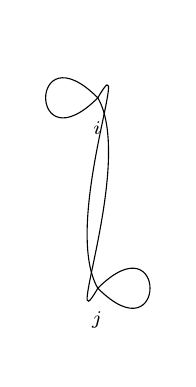
\begin{tikzpicture}[baseline={([yshift=0.2ex]current bounding box.center)}]
      \begin{feynman}
        \vertex (a);
        \vertex (b);
        \diagram {
          a -- [out=135, in=-135, loop, min distance=1.25 cm] a -- 
          [out=60, in=120] b -- [out=45, in=-45, loop, min distance=1.25cm] b 
          -- [out=-120, in=-60] a,
        };
        \vertex [below=0.5em of a] {\(_{i}\)};  
        \vertex [below=0.5em of b] {\(_{j}\)};  
      \end{feynman}
    \end{tikzpicture}
    + \frac{1}{48} 
    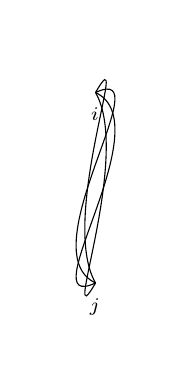
\begin{tikzpicture}[baseline={([yshift=0.2ex]current bounding box.center)}]
      \begin{feynman}
        \vertex (a);
        \vertex (b);
        \diagram {
          a -- 
          [out=60, in=120] b 
          -- [out=-120, in=-60] a,
          a -- [out=25, in=155] b 
          -- [out=-155, in=-25] a,
        };
        \vertex [below=0.2em of a] {\(_{i}\)};  
        \vertex [below=0.2em of b] {\(_{j}\)};  
      \end{feynman}
    \end{tikzpicture}
    \right]\, .
\end{align}
It it clear from the diagrammatic representation that we can
distinguish connected and disconnected contributions. The connected
contributions are represented by connected diagrams, i.e. diagrams
that are made of a single line. The disconnected diagrams are products
of multiple connected parts, and therefore correspond to products of
independent sums over subset of indices. In
Eq.~\ref{eq:PhiFourPartitionFuncOrderLambdaTwo} only the first term in
the bracket in the second line is a disconnected contribution. 

\paragraph{Connected contribution}

Using the Taylor expansion for the logarithm,
\begin{equation}
  \label{eq:TaylorLog}
  \log(1+x) = \sum_{n=1}^\infty (-)^{n+1} \frac{x^n}{n}\, ,
\end{equation}
we can compute
\begin{align}
  \label{eq:PhiFourPartitionFuncConnectOrderLambdaTwo}
  \log\left(Z(\lambda)/Z(0)\right) = 
                    &- \lambda \frac{1}{8} \sum_{i=1}^n \Delta_{ii}^2
                                     +\nonumber \\
                     &+\lambda^2
                    \left[
                    \frac{1}{128} \sum_i \Delta_{ii}^2 \sum_j \Delta_{jj}^2 +
                    \frac{1}{16} \sum_{ij} \Delta_{ii} \Delta_{jj} \Delta_{ij}^2 +
                    \frac{1}{48} \sum_{ij} \Delta_{ij}^4
                    \right] -  \nonumber \\
  &- \lambda^2 \frac{1}{2} \left( - \frac{1}{8}
    \sum_{i=1}^n \Delta_{ii}^2\right)^2 +  O(\lambda^3)\, . 
\end{align}
Eq.~\ref{eq:PhiFourPartitionFuncConnectOrderLambdaTwo} shows
explicitly the cancellation at order $\lambda^2$ between the first
term in the square bracket in the second line, and the last term in
the third line, which comes from squaring the order $\lambda$
contribution when computing the second term in the Taylor expansion in
Eq.~\ref{eq:TaylorLog}. This is a general property, taking the
logarithm of the generating function yields the generating function of
connected conributions. We shall prove this property later in the
course. 

\section{Perturbed Gaussian Correlators}
\label{sec:pert-gauss-corr}

The perturbative treatment discussed above can be extended to compute
moments of the distribution:
\begin{equation}
  \label{eq:lPointCorrPert}
  \langle x_{i_1} \ldots x_{i_\ell}\rangle =
  \frac{1}{Z(\lambda)} 
  \int d^nx\, e^{-S(x;\lambda)} x_{i_1} \ldots x_{i_\ell}\, ,
\end{equation}
which often referred to as an $\ell$-point correlator/function. Let us start
our discussion with a simple example. 

\paragraph{Two-point function}

We need to evaluate
\begin{align}
  \int d^nx\, e^{-S(x;\lambda)} x_{i_1} x_{i_2} &= 
  \int d^nx\, e^{-S_0(x;\lambda)}\, \left[\sum_{k=0}^\infty
  \frac{(-)^k}{k!} \lambda^k V(x)^k \right]\, x_{i_1} x_{i_2} \\
  \label{eq:TwoPointCorrPert}
                                               &=Z(0) \sum_{k=0}^\infty
  \frac{(-)^k}{k!} \lambda^k \langle V(x)^k x_{i_1} x_{i_2}\rangle_0\, ,
\end{align}
where in the second line we have expressed the initial correlator in
terms of correlators computed in the Gaussian theory, denoted as
before by $\langle \ldots \rangle_0$. The Gaussian correlators can be
computed using Wick's theorem as before. We shall consider again a
quartic potential:
\begin{equation}
  V(x) = \frac{1}{4!} \sum_{i=1}^n x_i^4\, ,
\end{equation}
and compute all the terms in Eq.~\ref{eq:TwoPointCorrPert} order by
order in $\lambda$ up to order $\lambda^2$.
\begin{itemize}
\item $O(\lambda^0)$ For $k=0$ we simply get the two-point Gaussian
  correlator: 
  \begin{align}
    \langle x_{i_1} x_{i_2} \rangle_0 = \Delta_{i_1 i_2}\, .
  \end{align}
\item $O(\lambda^1)$ At first order in $\lambda$ we have one insertion
  of $V$:
  \begin{align}
    \langle V(x) x_{i_1} x_{i_2} \rangle_0 = \frac{1}{4!} \sum_{i=1}^n
    \langle x_i^4 x_{i_1} x_{i_2} \rangle_0\, .
  \end{align}
  This Gaussian expectation value involving six factors of $x$ (four
  from the potential, and the two coming from the fact that we compute
  a two-point function) can be evaluated using Wick's
  theorem. There two types of contractions.
  \begin{itemize}
  \item [(i)] $x_1$ is contracted with $x_2$, and the four $x_i$ are
    contracted amongst themselves:
    \begin{align}
      \contraction{}{x_{i_1}}{}{x_{i_2}}
      x_{i_1} x_{i_2} 
      \left(
      \contraction{}{x_{i}}{}{x_{i}}
      \contraction{x_{i} x_{i}}{x_{i}}{}{x_{i}}
      x_{i} x_{i} x_{i} x_{i} +
      \contraction{}{x_{i}}{x_{i}}{x_{i}}
      \contraction[2ex]{x_{i}}{x_{i}}{ x_{i}}{x_{i}}
      x_{i} x_{i} x_{i} x_{i} +
      \contraction{}{x_{i}}{x_{i}x_{i}}{x_{i}}
      \contraction[2ex]{x_{i}}{x_{i}}{}{x_{i}}
      x_{i} x_{i} x_{i} x_{i} 
      \right) = \Delta_{i_1 i_2} \langle x_i^4\rangle_0
      \, ,
    \end{align}
    where we have used the fact that the term inside the bracket on
    the LHS is simply $\langle x_i^4\rangle_0$ --
    cfr. Eq.~\ref{eq:FourPtGaussContract}.
  \item [(ii)] $x_1$ and $x_2$ are contracted with some of the $x_i$;
    there are 12 such contractions:
    \begin{align}
      \contraction{}{x_{i_1}}{x_{i_2}}{x_{i}}
      \contraction[2ex]{x_{i_1}}{x_{i_2}}{x_{i}}{x_{i}}
      x_{i_1} x_{i_2}  x_{i} x_{i} x_{i} x_{i} + \ldots = 
      \Delta_{i i_1} \Delta_{i i_2} \Delta_{i i} \times 4
      \times 3\, .
    \end{align}
  \end{itemize}
  Collecting all terms yields
  \begin{align}
   \frac{1}{4!} \sum_{i=1}^n
    \langle x_i^4 x_{i_1} x_{i_2} \rangle_0 = 
    \Delta_{i_1 i_2} \frac{1}{4!} \sum_{i=1}^n \langle x_i^4\rangle_0
    + \frac{1}{4!} \times 4 \times 3 \sum_{i=1}^n \Delta_{i i_1}
    \Delta_{i i_2} \Delta_{i i} \, .
  \end{align}
\item $O(\lambda^2)$ At this order we need to evaluate
  \begin{align}
    \frac{1}{2!} \langle V(x)^2 x_{i_1} x_{i_2} \rangle_0 = 
    \frac{1}{2!} \frac{1}{(4!)^2} \sum_{i,j=1}^n \langle x_i^4 x_j^4
    x_{i_1} x_{i_2} \rangle_0\, .
  \end{align}
  There are five different types of contractions, each of them coming
  with a given multiplicity. We encourage the interested reader to
  compute those contributions, and check carefully that the correct
  multiplicities are recovered. 
\end{itemize}
Collecting all contributions yields
\begin{align}
  \int d^nx\, e^{-S(x;\lambda)} 
  x_{i_1} x_{i_2} = Z(0) & 
                           \left[
                           \Delta_{i_1 i_2} - \lambda \left(\Delta_{i_1 i_2}
                           \frac{1}{4!} \sum_{i=1}^n \langle
                           x_i^4\rangle_0 +  \frac12 \sum_{i=1}^n
                           \Delta_{i i_1} \Delta_{i i_2} \Delta_{i i} 
                           \right) + \right. \nonumber \\
                         & \left.
                           + \lambda^2 \left( 
                           \frac{1}{2!} \Delta_{i_1 i_2} \frac{1}{(4!)^2}
                           \sum_{i,j=1}^n \langle x_i^4 x_j^4 \rangle_0
                           + \frac{1}{2!} \sum_{i=1}^n \Delta_{i i_1}
                           \Delta_{i i_2} \Delta_{i i}  \frac{1}{4!}
                           \sum_{j=1}^n \langle x_j^4 \rangle_0
                           + \right. \right. \nonumber \\
                         & + \left. \left.
                           \frac{1}{4} \sum_{i,j=1}^n \Delta_{i i_1}
                           \Delta_{i i_2} \Delta_{i j}^2 \Delta_{jj}
                           + \frac{1}{6} \sum_{i,j=1}^n \Delta_{i i_1}
                           \Delta_{j i_2} \Delta_{i j}^3 +
                           \right. \right. \nonumber \\
  \label{eq:TwoPointNotNorm}
                         & + \left. \left.
                           \frac{1}{4} \sum_{i,j=1}^n \Delta_{i i_1}
                           \Delta_{j i_2} \Delta_{i j} \Delta_{ii}\Delta_{jj}
                           \right)
                           \right]\, .
\end{align}
Diagrammatically we have: 
\begin{align}
  \label{eq:TwoPtVacuumIncluded}
  \langle x_{i_1} x_{i_2}\rangle = 
  \frac{Z(0)}{Z(\lambda)} \Bigg[
    \begin{tikzpicture}[baseline={([yshift=1.4ex]current bounding box.center)}]
    \begin{feynman}[inline=(a)]
      \vertex (a);
      \vertex (b);
      \diagram {
        a -- b,
      };
      \vertex [below=0.2em of a] {\(_{i_1}\)};  
      \vertex [below=0.2em of b] {\(_{i_2}\)};  
    \end{feynman}
  \end{tikzpicture}
  + \frac{\lambda}{8}
    \begin{tikzpicture}[baseline={([yshift=-5ex]current bounding box.center)}]
    \begin{feynman}[layered layout, vertical'=i to c]
      \vertex (a);
      \vertex (c); 
      \vertex (b);
      \vertex (i);
      \vertex (j);
      \vertex (k);
      \diagram {
        j -- [draw=none]  i -- [draw=none] k, 
        i -- [out=45, in=-45, loop, min distance=2cm] i --
        [out=135, in=-135, loop, min distance=2 cm] i,
        a -- c -- b, 
        c --[opacity=0.1] i, 
      };
      \vertex [below=0.2em of a] {\(_{i_1}\)};  
      \vertex [below=0.2em of b] {\(_{i_2}\)};  
%      \vertex [below=0.2em of c] {\(c\)};  
      \vertex [below=0.2em of i] {\(_{i}\)};  
    \end{feynman}
  \end{tikzpicture}
  + \frac{\lambda}{2}
    \begin{tikzpicture}[baseline={([yshift=-3ex]current bounding box.center)}]
    \begin{feynman}[layered layout, vertical'=i to c]
      \vertex (a);
      \vertex (b);
      \vertex (i);
      \diagram {
        a -- i -- b, 
        i -- [out=135, in=45, loop, min distance=2cm] i,
      };
      \vertex [below=0.2em of a] {\(_{i_1}\)};  
      \vertex [below=0.2em of b] {\(_{i_2}\)};  
%      \vertex [below=0.2em of c] {\(c\)};  
      \vertex [below=0.2em of i] {\(_{i}\)};  
    \end{feynman}
  \end{tikzpicture}
  + O(\lambda^2)
  \Bigg]\, ,
\end{align}
where for simplicity we have omitted the contribution of order
$\lambda^2$. A diagram that can be factorised as the product of a
subdiagram with external lines and a subdiagram that is made of loops
only is called a {\em vacuum contribution}. For instance the second
diagram inside the bracket in Eq.~\ref{eq:TwoPtVacuumIncluded} is a
vacuum contribution, while the first and third ones are not.

Finally, we need to divide this expression by $Z(\lambda)$ in order to
obtain the two-point correlator as defined in
Eq.~\ref{eq:lPointCorrPert}.  As a result, we obtain a factor of
$Z(0)/Z(\lambda)$ multiplying the expression inside the square bracket
in Eq.~\ref{eq:TwoPointNotNorm}. Inverting
Eq.~\ref{eq:PhiFourPartitionFuncOrderLambdaTwo} for the ratio
$Z(0)/Z(\lambda)$ yields
\begin{align}
 Z(0)/Z(\lambda) &= 
                    1 + \frac{1}{4!} \lambda \sum_{i=1}^n \langle x_i^4\rangle_0 
                    - \frac{1}{2!} \frac{1}{(4!)^2} \lambda^2 \sum_{i,j=1}^n 
                    \langle x_i^4 x_j^4\rangle_0 
                   + \frac{1}{(4!)^2} \lambda^2 \left(\sum_{i=1}^n \langle x_i^4\rangle_0\right)^2
                   + O(\lambda^3) 
\end{align}

\begin{Ex}
  Show that all the vacuum contributions cancel when computing $\langle
  x_{i_1} x_{i_2}\rangle$. The final result is
  \begin{align}
  \int d^nx\, e^{-S(x;\lambda)} 
  x_{i_1} x_{i_2} = Z(0) & 
                           \left[
                           \Delta_{i_1 i_2} - \lambda  \frac12 \sum_{i=1}^n
                           \Delta_{i i_1} \Delta_{i i_2} \Delta_{i i} 
                            + \right. \nonumber \\
                         & \left.
                           + \lambda^2 \left( 
                           \frac{1}{4} \sum_{i,j=1}^n \Delta_{i i_1}
                           \Delta_{i i_2} \Delta_{i j}^2 \Delta_{jj}
                           + \frac{1}{6} \sum_{i,j=1}^n \Delta_{i i_1}
                           \Delta_{j i_2} \Delta_{i j}^3 +
                           \right. \right. \nonumber \\
  \label{eq:TwoPointNorm}
                         & + \left. \left.
                           \frac{1}{4} \sum_{i,j=1}^n \Delta_{i i_1}
                           \Delta_{j i_2} \Delta_{i j} \Delta_{ii}\Delta_{jj}
                           \right)
                           \right]\, .
\end{align}
Write a diagrammatic representation for the contributions $O(\lambda^2)$.
\end{Ex}
This is a general property: when the integral is divided by the
correct normalization factor $1/Z(\lambda)$, all vacuum contributions
cancel.

\section{Generating Functions for the Perturbed Gaussian Measure}
\label{sec:gener-funct-pert}

\paragraph{Correlators}

We can now generalise the idea of a generating function to the case of
a non Gaussian measure. Introducing
\begin{equation}
  \label{eq:GenFunctPert}
  Z(b;\lambda) = \int d^nx\, \exp\left[
    -S(x;\lambda) + (b,x)
    \right]\, ,
\end{equation}
where we introduced the notation
\begin{equation}
  \label{eq:ScalProd}
  (b,x) = \sum_{i=1}^n b_i x_i\, .
\end{equation}
Note that we can also write
\begin{equation}
  \label{eq:GenFunctPertTwo}
  \langle e^{(b,x)} \rangle = Z(b;\lambda)/Z(\lambda)\, .
\end{equation}
The correlators in the perturbed measure are obtained by
differentiation
\begin{equation}
  \label{eq:CorrGenPert}
  \langle x_{i_1} \ldots x_{i_\ell}\rangle = \frac{1}{Z(\lambda)} \left.
  \frac{\partial}{\partial b_{i_1}} \ldots \frac{\partial}{\partial b_{i_\ell}}\,
  Z(b;\lambda)
\right|_{b=0} \, .
\end{equation}

\paragraph{Cumulants}

The logarithm of $Z(b;\lambda)$ is usually denoted $W(b;\lambda)$, 
\begin{equation}
  \label{eq:WGenDef}
  Z(b;\lambda) = e^{W(b;\lambda)}\, ;
\end{equation}
$W(b;\lambda)$ is the generator is the generator of the connected
$\ell$-point correlators, $W_{i_1 \ldots i_\ell}$, i.e. the correlators that can be represented as a single
diagram, with $\ell$ open ends:
\begin{equation}
  \label{eq:DiffWGen}
  W_{i_1 \ldots i_\ell} = \left.
  \frac{\partial}{\partial b_{i_1}} \ldots \frac{\partial}{\partial b_{i_\ell}}\,
  W(b;\lambda)
\right|_{b=0} \, .
\end{equation}
In statistics, the $W_{i_1 \ldots i_\ell}$ are called the {\em
  cumulants} of the probability distribution $e^{-S(x;\lambda)}$.





\chapter{Path Integrals in QM}
\label{chap:lec1}
\newcommand{\epsstep}{\left(e^{-i \hat{H} \epsilon}\right)}

\section{Preliminaries}
\label{sec:preliminaries-1}

In this lecture we introduce Path Integrals in the context of
QM. Despite the simpler setting (QM compared to QFT), all the
important features of Path Integrals will be discussed. We consider a
point particle in one-dimension, and denote by $\hat{Q}$ the position
operator, and by $\ket{q}$ the eigenstate corresponding to the eigenvalue
$q$:
\begin{equation}
  \label{eq:QEigen}
  \hat{Q} \ket{q} = q \ket{q}\, .
\end{equation}
The completeness condition for the states $\ket{q}$ is
\begin{equation}
  \label{eq:qComplete}
  \int dq\, \ket{q}\bra{q} = 1\, .
\end{equation}
The aim of this section is to find an expression for the quantum
amplitude $\braket{q't'}{qt}$ for a system in state $\ket{q}$ at time
$t$ to evolve in state $\ket{q'}$ at time $t'$,
\begin{equation}
  \label{eq:AmplitudeDef}
  \braket{q't'}{qt} = \langle q' | e^{-i \hat{H} (t'-t)}|q\rangle\, ,
\end{equation}
where $\hat{H}$ is the Hamiltonian of the system. 

\section{Setting Up the Path Integral}
\label{sec:setting-up-path}

In order to proceed with the calculation, let us define $T=t'-t$ to be
the size of the time interval, and $\epsilon=T/n$, where $n$ is an
integer. Then 
\begin{align}
  t_0 &= t \\
  t_k &= t_0 + k \epsilon, \quad \text{for}\ k=1, \ldots, n-1 \\
  t_n &= t + n \epsilon = t'\, .
\end{align}
\begin{align}
  \langle q' | e^{-i \hat{H} (t'-t)}|q\rangle &= 
                 \langle q' | e^{-i \hat{H} T} | q\rangle \\
               &= \langle q' | \left(e^{-i \hat{H} \epsilon}\right)
                 \ldots \left(e^{-i \hat{H} \epsilon}\right) |
                 q\rangle\, ,
\end{align}
where the expression in the second line contains $n$ factors. 

Inserting the completeness relation $n-1$ times,
\begin{align}
  \label{eq:AmplitudeStepOne}
  \braket{q't'}{qt} = \int \prod_{k=1}^{n-1}dq_k\,
  \langle q' | \left(e^{-i \hat{H} \epsilon}\right) |q_{n-1}\rangle
  \langle q_{n-1} | \left(e^{-i \hat{H} \epsilon}\right) |
  q_{n-2}\rangle \ldots \langle q_1 | \left(e^{-i \hat{H}
  \epsilon}\right) | q\rangle\, .
\end{align}
For small $\epsilon$ we can expand the exponential to first order and
evaluate the matrix elements:
\begin{align}
  e^{-i \hat{H} \epsilon} &= 1 - i \hat{H} \epsilon + O(\epsilon^2)\\
\hat{H} &= \frac12 \hat{P}^2 + V(\hat{Q})\, ,
\end{align}
From the potential energy we get
\begin{align}
  \langle q_k | V(\hat{Q}) | q_{k-1}\rangle &= V(q_{k-1}) \langle q_k
                                              | q_{k-1} \rangle \\
                                            &= V\left(\frac{q_k +
                                              q_{k-1}}{2}\right)
                                              \delta(q_k-q_{k-1}) \\
                                            & = \int \frac{dp}{2\pi} V\left(\frac{q_k +
                                              q_{k-1}}{2}\right) 
                                              e^{ip (q_k-q_{k-1})}
\end{align}
In order to evaluate the contribution of the kinetic term, we
introduce eigenstates of the momentum operator $\ket{p}$
\begin{align}
  \hat{P} \ket{p} = p \ket{p} \\
  \braket{q}{p} = e^{ipq}\, ,
\end{align}
and use the completeness of the states $\ket{p}$:
\begin{align}
  \langle q_k | \hat{P}^2 | q_{k-1}\rangle = 
  \int \frac{dp_k}{2\pi}\, p^2 e^{ip_k(q_k-q_{k-1})}\, .
\end{align}
Hence
\begin{align}
  \langle q_k | e^{-i\hat{H}\epsilon} | q_{k-1}\rangle = 
  \int \frac{dp_k}{2\pi}\, \exp\left\{i\epsilon \left[
  p_k \frac{q_k-q_{k-1}}{\epsilon} - H\left(p_k,\tilde{q}_k\right)
  \right]
  \right\} + O(\epsilon^2)\, ,
\end{align}
where $\tilde{q}_k=\frac{q_k-q_{k-1}}{2}$. Therefore
\begin{align}
  \braket{q't'}{qt} =& \lim_{n\to\infty} \int \prod_{k=1}^{n-1}dq_k\, 
  \prod_{j=1}^{n} \frac{dp_j}{2\pi}\, \times \\
  &\times \exp \left\{
    i\epsilon \sum_{m=1}^{n} \left[
    p_m \frac{q_m-q_{m-1}}{\epsilon} - H\left(p_m, 
    \frac{q_m+q_{m-1}}{2}\right)
    \right]
    \right\}\, ,
\end{align}
where $q_0 = q$, and $q_n = q'$. The limit above defines the {\em
  path integral} evaluation of the quantum amplitude, which we denote 
\begin{align}
  \label{eq:PathIntDefZero}
  \braket{q't'}{qt} = 
  \int \mathcal{D}q \mathcal{D}p \exp \left\{
  i \int_t^{t'} d\tau\, \left[
  p \dot{q} - H(p,q)
  \right]
  \right\}\, .
\end{align}

\section{Quadratic P dependence}
\label{sec:quadr-kinet-term}

For hamiltonians like the one above, \ie hamiltonians that are only
quadratic in the momentum $\hat{P}$, the expression above can be
simplified by performing the integral over the momenta $p_j$:
\begin{align}
  \int \frac{dp}{2\pi}\, \exp\left\{
  i\epsilon\left[
  p \left(\frac{q_k-q_{k-1}}{\epsilon}\right) - \frac12 p^2
  \right]
  \right\} = \left(2\pi i \epsilon\right)^{-1/2}\,
  \exp\left\{i\epsilon
  \frac12\left(\frac{q_k-q_{k-1}}{\epsilon}\right)^2\right\}\, .
\end{align}
Using this result, we can rewrite the path integral in
\Eqref{eq:PathIntDefZero} as
\begin{align}
  \label{eq:PathIntDefOne}
  \braket{q't'}{qt} = \lim_{n\to\infty}
  \left(2\pi i \epsilon\right)^{-n/2}\,
  \int \prod_{k=1}^{n-1}dq_k\, 
  \exp \left\{
  i \epsilon \sum_{m=1}^{n}
  \, \left[
  \frac12 \left(\frac{q_m-q_{m-1}}{\epsilon}\right)^2
  -V\left(\frac{q_m+q_{m-1}}{2}\right)
  \right]
  \right\}\, .
\end{align}
Assuming that the limit exists, we have obtained the definition of the
path integral as an integral over the position of the system only: 
\begin{align}
  \label{eq:PathIntDef}
  \braket{q't'}{qt} = 
  \int_{q,q'} \mathcal{D}q \exp \left\{
  i \int_t^{t'} d\tau\,  \mathcal{L}(q,\dot{q})
  \right\}\, ,
\end{align}
where $\mathcal{L}$ is the lagrangian of the system. Note that the
suffix of the integral keeps track of the initial- and final-state
configurations $q$ and $q'$. 

\section{Correlators}
\label{sec:correlators}

We are now going to work out expressions for the matrix element of the
position operator inbetween the initial and final state considered
above. 

\subsection{One-point Function}
\label{sec:one-point-function}

The first example that we are going to consider is the matrix element
\begin{align}
  \label{eq:OnePtDef}
  \langle q't' | \hat{Q}(\bar{t}) | q t\rangle = 
  \langle q' | e^{-i \hat{H}(t'-t)} \hat{Q} e^{-i \hat{H}(\bar{t}-t)}
  | q\rangle\, ,
\end{align}
where we assume $t<\bar{t}<t'$, and we have used
\begin{equation}
  \label{eq:HeisenOpEvol}
  \hat{Q}(t) = e^{i\hat{H} t} \hat{Q} e^{-i\hat{H} t}\, .
\end{equation}
Proceeding as we did in the previous section, we can write
\begin{align}
  \label{eq:CorrOne}
  \langle q't' | \hat{Q}(\bar{t}) | q t\rangle = 
  \bra{q'} \epsstep \ldots \epsstep \hat{Q} \epsstep \ldots
  \epsstep \ket{q}\, ,
\end{align}
where we assumed that $\bar{t}=t_k$, and the first and second ellipses
denote respectively $(n-k)$, and $k$ factors of $\epsstep$. Performing
the same manipulations as before we obtain
\begin{align}
  \langle q't' | \hat{Q}(\bar{t}) | q t\rangle =& 
  \lim_{n\to\infty} \int \prod_{k=1}^{n-1}dq_k\, 
  \prod_{j=1}^{n} \frac{dp_j}{2\pi}\, q_k \times \\
  &\times \exp \left\{
    i\epsilon \sum_{m=1}^{n} \left[
    p_m \frac{q_m-q_{m-1}}{\epsilon} - H\left(p_m, 
    \frac{q_m+q_{m-1}}{2}\right)
    \right]
    \right\}\, .
\end{align}
Note that now there is an extra factor of $q_k$ in the integrand,
corresponding to the insertion of the operator $\hat{Q}(\bar{t})$. The
limit above  is denoted
\begin{align}
  \langle q't' | \hat{Q}(\bar{t}) | q t\rangle &= 
  \int \mathcal{D}q \mathcal{D}p \, q(\bar{t}) 
  \exp \left\{
  i \int_t^{t'} d\tau\, \left[
  p \dot{q} - H(p,q)
  \right]
  \right\}\\
&= \int_{qq'} \mathcal{D}q \, q(\bar{t}) 
  \exp \left\{
  i \int_t^{t'} d\tau\, \mathcal{L}(q,\dot{q})
  \right\}\, .
\end{align}

\subsection{Two-point function}
\label{sec:two-point-function}

Let us now consider the slightly more complicated case of the matrix
element of the product of two position operators
\begin{align}
  \label{eq:TwoPtDef}
  \bra{q't'} \hat{Q}(\bar{t}_1) \hat{Q}(\bar{t}_2)\ket{qt}\, , 
\end{align}
where now we assume $\bar{t}_1=t_k$, $\bar{t}_2=t_\ell$,
$t<\bar{t}_2<\bar{t}_1<t'$. We can write this correlator as:
\begin{align}
    \bra{q't'} \hat{Q}(\bar{t}_1) \hat{Q}(\bar{t}_2)\ket{qt} = 
  \bra{q'} \epsstep \dots \hat{Q} \ldots \hat{Q} \ldots \epsstep
  \ket{q}\, ,
\end{align}
where the three ellipses here denote respectively $(n-k)$, $(k-\ell)$,
and $\ell$ factors of $\epsstep$. Proceeding exactly as above yields: 
\begin{align}
  \label{eq:TwoPtPathInt}
  \bra{q't'} \hat{Q}(\bar{t}_1) \hat{Q}(\bar{t}_2)\ket{qt} = 
  \int_{qq'} \mathcal{D}q\, q(\bar{t}_1) q(\bar{t}_2) 
  \exp \left\{
  i \int_t^{t'} d\tau\, \mathcal{L}(q,\dot{q})
  \right\}\, .
\end{align}

There is a subtlety here that it is worth noting. The ordering of
times in \Eqref{eq:TwoPtDef} matters, while it clearly does not in the
RHS of \Eqref{eq:TwoPtPathInt} where $q(\bar{t}_1)$ and $q(\bar{t}_1)$
are just integration variables. If $\bar{t}_2>\bar{t}_1$, then the RHS
of \Eqref{eq:TwoPtPathInt} corresponds to
\begin{align}
  \bra{q't'} \hat{Q}(\bar{t}_2) \hat{Q}(\bar{t}_1) \ket{qt}\, .
\end{align}
Both results can be summarised as
\begin{align}
  \label{eq:TOrderPathInt}
  \bra{q't'} T\left(\hat{Q}(\bar{t}_1) \hat{Q}(\bar{t}_2)
  \right)\ket{qt} = 
  \int_{qq'} \mathcal{D}q\, q(\bar{t}_1) q(\bar{t}_2) 
  \exp \left\{
  i \int_t^{t'} d\tau\, \mathcal{L}(q,\dot{q})
  \right\}\, ,
\end{align}
where we have introduced the T-ordered product of operators: 
\begin{align}
  \label{eq:TOrderDef}
   T\left(\hat{Q}(t) \hat{Q}(t')\right) = \theta(t-t') \hat{Q}(t)
  \hat{Q}(t') + \theta(t'-t) \hat{Q}(t') \hat{Q}(t)\, .
\end{align}

You can easily verify that the derivation can be extended to
an arbitrary number of insertions of the operator $\hat{Q}$:
\begin{align}
\label{eq:TOrderNPt}
\bra{q't'} T\left(\hat{Q}(\bar{t}_1) \ldots \hat{Q}(\bar{t}_n)
  \right)\ket{qt} = 
  \int_{qq'} \mathcal{D}q\, q(\bar{t}_1) \ldots q(\bar{t}_n) 
  \exp \left\{
  i \int_t^{t'} d\tau\, \mathcal{L}(q,\dot{q})
  \right\}\, .
\end{align}

\section{Generating functional}
\label{sec:gener-funct}

\subsection{Functional derivative}
\label{sec:funct-deriv}

Consider a functional $F$ that associates a number, which we denote
$F[u]$, to a given function $u(x)$. The functional derivative
describes the change of the functional to an infinitesimal variation
of the function $u$: 
\[
  u(x) \mapsto u(x) + \delta u(x)\, .
\]
We define
\begin{equation}
  \label{eq:FuncDer}
  \delta F = F[u+\delta u] - F[u] = \int dx\, \frac{\delta F}{\delta
    u(x)} \delta u(x)\, .
\end{equation}
You can see the analogy to the case of a function of several
variables, where the variation to a change $\delta x_k$ in the
variables is given by
\begin{equation}
  \label{eq:NormDer}
  \delta F = F(x+\delta x) - F(x) = \sum_k \frac{\partial F}{\partial
    x_k} \delta x_k\, .
\end{equation}
In particular we have
\begin{equation}
  \label{eq:DiracDelta}
  \frac{\delta}{\delta f(x)} f(y) = \delta(x-y)\, , 
\end{equation}
again to be compared with its discrete analogue
\begin{equation}
  \label{eq:KroneckerDelta}
  \frac{\partial}{\partial x_j} x_i = \delta_{ij}\, .
\end{equation}

\subsection{Sources in the path integral}
\label{sec:sourc-path-integr}

Let $f(t)$ and $h(t)$ be two functions, we can add so-called source
terms to the path integral, and define
\begin{equation}
  \label{eq:PathIntegralSources}
  \braket{q't'}{qt}_{f,h} = \int \mathcal{D}p \mathcal{D}q\,\exp 
  \left\{
    i \int_{t}^{t'} d\tau \left[
      p(\tau) \dot{q}(\tau) - H(p(\tau),q(\tau)) + f(\tau) q(\tau) +
      h(\tau) p(\tau)
      \right]
  \right\}\, .
\end{equation}
Taking functional derivatives with respect to the source fields yields
e.g.
\begin{align}
  \left(\frac{1}{i} \frac{\delta}{\delta f(\bar\tau)} \right)&
  \braket{q't'}{qt}_{f,h} = \nonumber \\
  =&\int \mathcal{D}p \mathcal{D}q\,
  q(\bar{\tau})\,
  \exp \left\{
  i \int_{t}^{t'} d\tau \left[
  p(\tau) \dot{q}(\tau) - H(p(\tau),q(\tau)) + f(\tau) q(\tau) +
  h(\tau) p(\tau)
  \right]
  \right\}\, ,
\end{align}
\begin{align}
  \left(\frac{1}{i} \frac{\delta}{\delta f(\bar\tau_1)} \right)&
  \left(\frac{1}{i} \frac{\delta}{\delta f(\bar\tau_2)} \right)
  \braket{q't'}{qt}_{f,h} = \nonumber \\
  =&\int \mathcal{D}p \mathcal{D}q\,
  q(\bar{\tau}_1) q(\bar{\tau}_2)\,
  \exp \left\{
  i \int_{t}^{t'} d\tau \left[
  p(\tau) \dot{q}(\tau) - H(p(\tau),q(\tau)) + f(\tau) q(\tau) +
  h(\tau) p(\tau)
  \right]
  \right\}\, , 
\end{align}
and similarly for the derivatives with respect to $h$ pulling down
factors of $p$ in the integrand. 

As we have seen in the previous section, we have
\begin{align}
  \bra{q't'}  T\left(
  \hat{Q}(t_1)\ldots \hat{Q}(t_n) 
  \right)
  \ket{qt} =& \nonumber \\
  =& \left(\frac{1}{i} \frac{\delta}{\delta f(t_1)} \right) \ldots
    \left(\frac{1}{i} \frac{\delta}{\delta f(t_n)} \right)\,
    \braket{q't'}{qt}_{f,h}\Bigg|_{f=h=0}\, .
\end{align}

\section{Projection onto the ground state}
\label{sec:proj-onto-ground}

It is useful to be able to compute the amplitude for the system to
evolve from the vacuum state at time $t$ into the vacuum state at time
$t'$ under the action of the external sources $f,h$. Having computed
$\braket{q't'}{qt}$, the above amplitude is given by
\begin{align}
  \label{eq:VacToVacAmpl}
  \braket{0,t'}{0,t} = 
  \int dq dq'\, \phi_0(q')^*\, \braket{q't'}{qt}_{f,h}\, \phi_0(q)\, ,
\end{align}
where $\phi_0(q)=\braket{q}{0}$ is the wave function of the ground
state, and $\ket{n}$ denote the eigenstates of the
Hamiltonian. \Eqref{eq:VacToVacAmpl} yields the right amplitude, but
requires the convolution of $\braket{q't'}{qt}$ with the ground state
wave function. We shall now describe a procedure that allows the
compute the vacuum-to-vacuum amplitude directly as a path integral. 

The energy eigenstates are
\begin{equation}
  \label{eq:EnEigen}
  \hat{H} \ket{n} = E_n \ket{n}\, ,
\end{equation}
and their wave functions are denoted as
\begin{equation}
  \label{eq:EnEigenFun}
  \phi_n(q) = \braket{q}{n}\, .
\end{equation}
We assume that the vacuum energy vanishes, $E_0=0$. We want to
evaluate the amplitude
\begin{equation}
  \label{eq:LargeQAmpl}
  \braket{Q'T'}{QT}_{f,h}
\end{equation}
where the sources $h$ and $f$ have support in the interval $[t,t']$,
with $T < t < t' < T'$. The sources behind switched off between $T$
and $t$, we can readily compute
\begin{align}
  \braket{qt}{QT} &= \int \mathcal{D}q \mathcal{D}p \,
                    \exp\left\{
                    i \int_T^t d\tau\, \left[
                    p \dot{q} - H(p,q)
                    \right]
                    \right\} \\
  &= \bra{q} \exp\left[-i \hat{H} (t-T)\right] \ket{Q} \\
  &= \sum_n \phi_n(q) \phi_n(Q)^* e^{-i E_n(t-T)}\, .
\end{align}
We can now analytically continue the result to $T_I=(1-i\epsilon)T$,
and consider the limit $T\to -\infty$:
\begin{align}
  \lim_{T\to -\infty} \braket{qt}{QT_I} = \phi_0(q) \phi_0(Q)^*\, .
\end{align}
A similar result can be obtained for $\braket{Q'T'}{q't'}$. We can
therefore write
\begin{align}
  \braket{Q'T'}{QT}_{f,h} = \int dq' dq\, \braket{Q'T'}{q't'} \braket{q't'}{qt}_{f,h}
  \braket{qt}{QT}\, .
\end{align}
And therefore
\begin{align}
 \lim_{T'\to\infty,T\to -\infty} 
\frac{\braket{Q', (1-i\epsilon)T'}{Q, (1-i\epsilon)T}_{f,h}}{\phi_0(Q)^* \phi_0(Q')} = 
  \int dq dq'\, \phi_0(q')^* \braket{q't'}{qt}_{f,h} \phi_0(q)\, .
\end{align}
The expresson on the RHS is the vacuum-to-vacuum amplitude,
$\braket{0,t'}{0,t}_{f,h}$, that we want to compute. The expression on
the LHS is the limit of the path integral for $T\to\infty$,
$T'\to\infty$. The only dependence on the boundary values $Q$ and $Q'$
appears in the denominator on LHS: it is a normalization factor
independent of $f$ and $h$, which disappears when taking derivatives
with respect to the sources. Instead of analytically continuing to
complex values of $T$ and $T'$, we can simply add an imaginary part to
the Hamiltonian,
\begin{equation}
  \label{eq:ComplexTermHam}
  \hat{H} \to (1-i\epsilon) \hat{H}\, .
\end{equation}
Taking the limit $T\to\infty$, $T'\to\infty$, we obtain the amplitude
\begin{equation}
  \label{eq:VacToVac}
  \braket{0}{0}_{f,h} = \int \mathcal{D}p \mathcal{D}q \, \exp
  \left\{
    i \int_{-\infty}^\infty d\tau\, \Big[
      p \dot{q} - (1-i\epsilon) H(p,q) + f q + h p 
      \Big]
  \right\}
\end{equation}


\section{Weyl ordering}
\label{sec:weyl-ordering}

If we are interested in more general Hamiltonians, with terms that
involve products of $\hat{P}$ and $\hat{Q}$, then we need to give a
prescription for the ordering of the operators in the Hamiltonian, so
that the quantum mechanical amplitude is actually described by the
path integral. 

As discussed by Berezin in 1971, the mid-point prescription we adopted
in \Eqref{eq:PathIntDefOne} is equivalent to the Weyl-ordering of the
Hamiltonian. 

The Weyl product of two operators $\hat{A}$ and $\hat{B}$ is defined
by considering the operator $\left(\alpha \hat{A} + \beta
  \hat{B}\right)^n$, and expanding it in powers of $\alpha$ and $\beta$: 
\begin{equation}
  \label{eq:WeylOrder}
  \left(\alpha \hat{A} + \beta
    \hat{B}\right)^n = \sum_k \frac{n!}{k! l!}\, 
  \alpha^k \beta^l\, \left[\hat{A}^k
    \hat{B}^l\right]\, .
\end{equation}
The quantity in the square bracket is the Weyl ordered product of
$\hat{A}^k$ and $\hat{B}^l$. 



\chapter{Path Integrals for Scalar Fields}
\label{cha:path-integr-scal}

\section{Everything up to FD in mom space goes here}
\label{sec:everything-up-fd}

Everything up to Feynman diagrams in momentum space. 



\chapter{Path Integrals for Fermion Fields}
\label{cha:path-integr-ferm}

\chapter{Path Integrals for Gauge Fields}
\label{cha:path-integrals-gauge}

\chapter{Divergences I - the Scalar Propagator}
\label{cha:divergences-i-scalar}

\chapter{Divergences II - the Vertex Function}
\label{cha:diverg-ii-vert}

\chapter{Renormalization}
\label{cha:renormalization}

\section{Regularization}
\label{sec:regularization}

\section{Renormalization schemes}
\label{sec:renorm-schem}



\chapter{Renormalization Group}
\label{cha:renorm-group}

\chapter{Scales - Decoupling}
\label{cha:scales-decoupling}

\printindex
\end{document}

%%% Local Variables:
%%% mode: latex
%%% TeX-master: t
%%% End:
